\documentclass[conference,onecolumn]{IEEEtran}
\IEEEoverridecommandlockouts
% The preceding line is only needed to identify funding in the first footnote. If that is unneeded, please comment it out.
\usepackage{cite}
\usepackage{amsmath,amssymb,amsfonts}
\usepackage{algorithmic}
\usepackage{graphicx,subcaption}
\usepackage{float}
\usepackage{hyperref}
\usepackage{textcomp}
\usepackage{xcolor}
\usepackage{listings}
\usepackage{enumitem}

\DeclareMathOperator*{\argmax}{arg\,max}
\DeclareMathOperator*{\argmin}{arg\,min}

\def\BibTeX{{\rm B\kern-.05em{\sc i\kern-.025em b}\kern-.08em
    T\kern-.1667em\lower.7ex\hbox{E}\kern-.125emX}}

\IEEEoverridecommandlockouts

\lstset{
    language=MATLAB,             % Set language to MATLAB
    basicstyle=\ttfamily\small,  % Set font to small and monospaced
    keywordstyle=\color{blue},   % Color keywords
    stringstyle=\color{green},   % Color strings
    commentstyle=\color{gray},   % Color comments
    showstringspaces=false,      % Do not display string spaces
    frame=single,                % Add a frame around the code
    breaklines=true              % Line breaks for long lines
}

\begin{document}

\title{\Large Assignment 3 --- Math Fundamentals for Robotics 16-811, Fall 2024}

\author{
      \IEEEauthorblockN{Mukai Yu}
      \IEEEauthorblockA{\textit{MSR, CMU} \\
            Pittsburgh, PA\\
            \href{mailto:mukaiy@andrew.cmu.edu}{mukaiy@andrew.cmu.edu}}
}

\maketitle

\begin{enumerate}[label=\arabic{enumi}.]
      \item Consider the function $f (x) = sin x - 0.5$ over the interval $[-\frac{\pi}{2}, \frac{\pi}{2}]$.
            \begin{enumerate}
                  \item What is the Taylor series expansion for $f (x)$ around $x = 0$ ?

                        \textbf{Solution:}
                        \begin{align*}
                              F(x) & = -0.5 + \sum_{k = 0}^\infty \frac{(-1)^k}{(2k + 1)!} x^{2k + 1}               \\
                                   & \approx -0.5 + x - \frac{x^3}{6} + \frac{x^5}{120} - \frac{x^7}{5040} + \cdots
                        \end{align*}
                  \item Graph $f (x)$ over the interval $[-\frac{\pi}{2}, \frac{\pi}{2}]$.

                        \textbf{Solution:}
                        \begin{figure}[H]
                              \centering
                              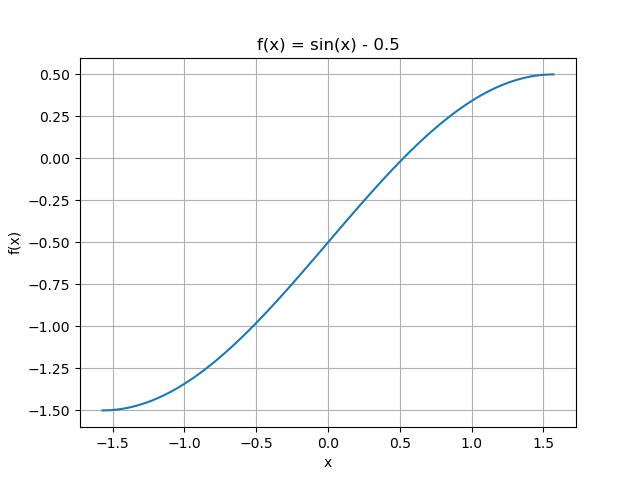
\includegraphics[width=0.5\linewidth]{figs/Q1.png}
                              \caption{Graph of $f(x) = sin (x) - 0.5$}
                        \end{figure}
                  \item Determine the best uniform approximation by a quadratic to the function $f (x)$ on the interval $[-\frac{\pi}{2}, \frac{\pi}{2}]$.
                        What are the $L_{\infty}$ and $L_2$ errors for this approximation?

                        \textbf{Solution:}

                        $n = 2$ so we need $n + 2 = 4$ points to determine the coefficients of the quadratic.
                        Let them be $\{x_0, x_1, x_2, x_3\}$, and let the quadratic function be $p_2(x) = a x^2 + b x + c$.

                        $f^{(n + 1)}(x) = f^{(3)}(x) = - cos(x)$ which doesn't change sign in $[-\frac{\pi}{2}, \frac{\pi}{2}]$, so by the theorem taught in class we know that:
                        \begin{align*}
                               & \begin{cases}
                                    x_0 = -\frac{\pi}{2} \\
                                    x_3 = \frac{\pi}{2}  \\
                                    e(x_0) = - e(x_1) = e(x_2) = - e(x_3) = E
                              \end{cases} \\
                               & +                         \\
                               & \begin{cases}
                                    e(x_0) = f(x_0) - p_2(x_0) = f(-\frac{\pi}{2}) - p_2(-\frac{pi}{2}) & = -1.5 - \frac{\pi^2}{4}a + \frac{\pi}{2}b - c \\
                                    e(x_1) = f(x_1) - p_2(x_1)                                          & = sin(x_1) - 0.5 - a x_1^2 - b x_1 - c         \\
                                    e(x_2) = f(x_2) - p_2(x_2)                                          & = sin(x_2) - 0.5 - a x_2^2 - b x_2 - c         \\
                                    e(x_3) = f(x_3) - p_2(x_3) = f(\frac{\pi}{2}) - p_2(\frac{\pi}{2})  & = 0.5 - \frac{\pi^2}{4}a - \frac{\pi}{2}b - c
                              \end{cases} \\
                               & +                         \\
                               & \begin{cases}
                                    e'(x_1) & = f'(x_1) - p_2'(x_1) = cos(x_1) - 2 a x_1 - b = 0 \\
                                    e'(x_2) & = f'(x_2) - p_2'(x_2) = cos(x_2) - 2 a x_2 - b = 0
                              \end{cases} \\
                               & \Downarrow                \\
                               & \begin{cases}
                                    c = -\frac{\pi^2}{4}a - 1 \\
                                    b = \frac{2E - 2}{\pi}
                              \end{cases}
                        \end{align*}
                        Now we see that the solution is not trivial, so we resort to numerical method \href{https://youtu.be/j29rVHCpRUY?si=eV1INsW6upgQ4lG5}{Remez Exchange Algorithm} to solve for the coefficients.
                        \begin{lstlisting}[language=Python]
def remez_exchange(
f, n: int, interval: list, max_num_iteration: int = 100, tolerance: float = 1e-5
):
      """Remez Exchange Algorithm

      Args:
            f (_type_): univariate function
            n (int): polynomial degree
            interval (list): interval for uniform approximate
            max_num_iteration (int): max number of iteration
            tolerance (float): tolerance of point change between updates
      """

      assert len(interval) == 2, "Interval must be a list of 2 elements"

      # we need n + 2 points to construct a polynomial of degree n, uniform initialization
      xi = np.linspace(interval[0], interval[1], n + 2)

      # define x
      x = sp.symbols("x", real=True)

      # numerical function f
      f_numerical = sp.lambdify(x, f, "numpy")

      # determine if f^(n + 1) does not change sign in the interval
      f_n_plus_1 = sp.diff(f, x, n + 1)
      roots = find_all_roots(sp.lambdify(x, f_n_plus_1, "numpy"), interval)

      if len(roots) == 0:
            print("f^(n + 1) does not change sign in the interval")
            xi[0] = interval[0]
            xi[-1] = interval[1]

      # # some turbulence in the initial points
      # xi[1] = -1.0

      for iter in range(max_num_iteration):
            print(f"\nIteration {iter}\n")

            # construct linear system
            A = np.ones((n + 2, n + 2))
            for degree in range(n + 1):
                  A[:, degree] = xi**degree
            A[:, -1] = (-1) ** np.arange(n + 2)

            b = f_numerical(xi).reshape(-1, 1)

            print(f"xi: {xi}")
            print(f"A: {A}")
            print(f"b: {b}")

            # solve linear system
            solution = np.linalg.solve(A, b).flatten()

            print(f"solution: {solution}")

            poly_coeff = solution[:-1]
            error = np.abs(solution[-1])

            # construct polynomial function with sympy
            poly = 0
            for degree in range(n + 1):
                  poly += poly_coeff[degree] * x**degree

            print("Polynomial function:")
            sp.pprint(poly)

            # find the maximum error
            error_func = f - poly
            error_func_numerical = sp.lambdify(x, error_func, "numpy")
            max_error_abs, max_point = find_max(error_func, interval)
            print(f"max error: {max_error_abs}")
            print(f"max point: {max_point}")

            # filter out the points with the same sign as the maximum error
            xi_new = xi.copy()
            xi_same_sign = xi_new[
                  np.where(
                  np.sign(error_func_numerical(xi_new))
                  == np.sign(error_func_numerical(max_point))
                  )
            ]

            # find the closest point to the maximum error point and replace it with the maximum error point
            closest_point = xi_same_sign[np.argmin(np.abs(xi_same_sign - max_point))]
            xi_new[np.where(xi_new == closest_point)] = max_point

            print(f"xi_new: {xi_new}")

            # if the error changing is less than tolerance, break the loop
            if np.abs(np.abs(error) - max_error_abs) < tolerance:
                  print(f"Converged after {iter} iterations")
                  break

            xi = np.sort(xi_new)

      if iter == max_num_iteration - 1:
            print(f"Did not converge after {max_num_iteration} iterations")

      return poly, poly_coeff, max_error_abs
                        \end{lstlisting}
                        \begin{figure}[H]
                              \centering
                              \begin{subfigure}{0.49\linewidth}
                                    \centering
                                    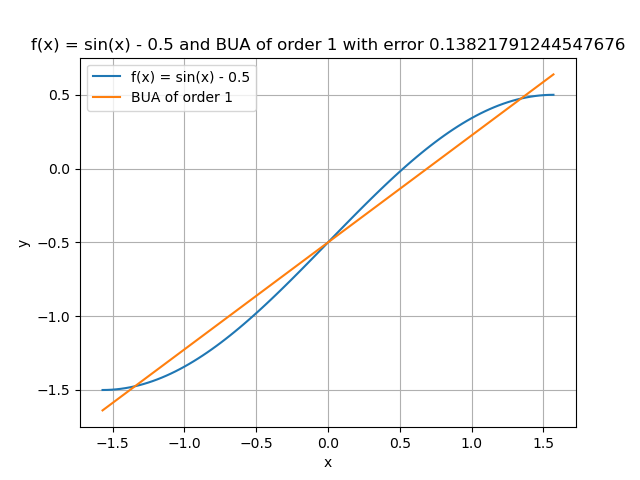
\includegraphics[width=\linewidth]{figs/Q1_c_poly_1.png}
                                    \caption{$n = 1$}
                              \end{subfigure}
                              \begin{subfigure}{0.49\linewidth}
                                    \centering
                                    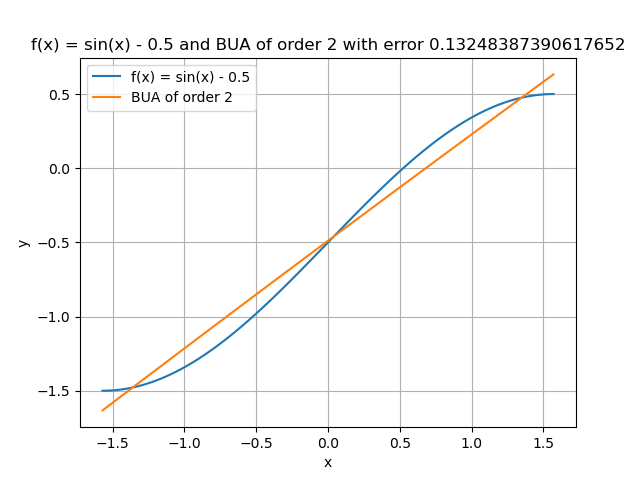
\includegraphics[width=\linewidth]{figs/Q1_c_poly_2.png}
                                    \caption{$n = 2$}
                              \end{subfigure} \\
                              \begin{subfigure}{0.49\linewidth}
                                    \centering
                                    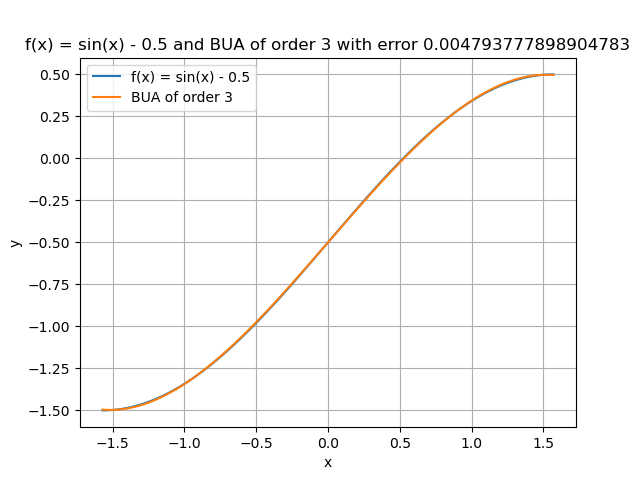
\includegraphics[width=\linewidth]{figs/Q1_c_poly_3.png}
                                    \caption{$n = 3$, error change does not converge to $< 10^{-5}$ in 1000 iterations}
                              \end{subfigure}
                              \begin{subfigure}{0.49\linewidth}
                                    \centering
                                    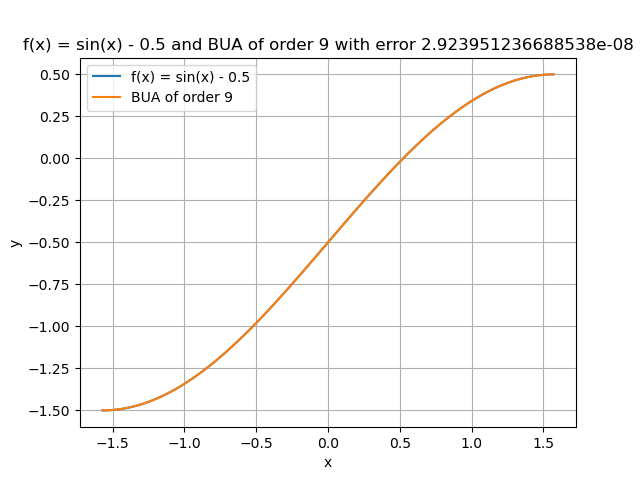
\includegraphics[width=\linewidth]{figs/Q1_c_poly_9.png}
                                    \caption{$n = 9$}
                              \end{subfigure}
                              \caption{Best Uniform Approximation using the Remez Exchange Algorithm}
                        \end{figure}

                        Well, I guess odd function approximation can get good results.

                        For $n = 1$:
                        \begin{align*}
                              \begin{cases}
                                    p_1(x)   & \approx 0.72460996019333 x - 0.5 \\
                                    L_\infty & \approx 0.13821791244547676      \\
                                    L_2      & \approx 0.170396813894351
                              \end{cases}
                        \end{align*}

                        For $n = 2$:
                        \begin{align*}
                              \begin{cases}
                                    p_2(x)   & \approx - 0.500004924940155 + 0.724609736054229 x + 1.9960030637173 \times 10^{-6} x^2 \approx 0.724609736054229 x - 0.5 \\
                                    L_\infty & \approx 0.13822185392370312                                                                                              \\
                                    L_2      & \approx 0.170396982005513
                              \end{cases}
                        \end{align*}

                        For $n = 3$:

                        Its error change does not converge to $< 10^{-5}$ in 1000 iterations
                        \begin{align*}
                              \begin{cases}
                                    p_3(x)   & \approx - 0.5000619896739 + 0.985440080596674 x + 0.000139910675817895 x^2 + 0.142443200483762 x^3 \\
                                    L_\infty & \approx 0.004793777898904783                                                                       \\
                                    L_2      & \approx 0.00568482890288639
                              \end{cases}
                        \end{align*}
                  \item Determine the best least-squares approximation by a quadratic to the function $f (x)$ over the interval $[-\frac{\pi}{2}, \frac{\pi}{2}]$.
                        What are the $L_{\infty}$ and $L_2$ errors for this approximation?

                        \textbf{Solution:}

                        Using Legendre polynomials as basis functions, we can solve for the coefficients of the quadratic.

                        Legendre polynomials modified for interval $[-\frac{\pi}{2}, \frac{\pi}{2}]$ has the following dot product definition:

                        $$
                              <f, g> = \int_{-\frac{\pi}{2}}^{\frac{\pi}{2}} f(x) g(x) dx
                        $$
                        Then with the first 2 Legendre polynomials:
                        \begin{align*}
                              \begin{cases}
                                    P_0(x) & = 1 \\
                                    P_1(x) & = x
                              \end{cases}
                        \end{align*}
                        We can derive more Legendre polynomials using the following recurrence relation:
                        $$
                              P_{n + 1}(x) = \left[ x - \frac{<x P_n(x), P_n(x)>}{<P_n(x), P_n(x)>}\right] P_n(x) - \frac{<P_n(x), P_n(x)>}{<P_{n - 1}(x), P_{n - 1}(x)>} P_{n - 1}(x), n = 1, 2, \cdots
                        $$
                        More Legendre polynomials:
                        \begin{align*}
                              \begin{cases}
                                    P_2(x) & = x^2 - \frac{\pi^2}{12}                                                       \\
                                    P_3(x) & = x^3 - \frac{3\pi^2}{20} x                                                    \\
                                    P_4(x) & = x^4 - \frac{3\pi^2}{14} x^2 + \frac{3\pi^4}{560}                             \\
                                    P_5(x) & = x^5 - \frac{5\pi^2}{18} x^3 + \frac{5\pi^4}{336} x                           \\
                                    P_6(x) & = x^6 - \frac{15\pi^2}{44} x^4 + \frac{5\pi^4}{176} x^2 - \frac{5\pi^6}{14784}
                              \end{cases}
                        \end{align*}
                        Now after projecting $f(x)$ onto the first 3 Legendre polynomials for quadratic least square approximation, we can solve for the coefficients of the quadratic.
                        \begin{align*}
                              f(x)     & \approx -0.5 P_0(x) + \frac{24}{\pi^3} P_1(x) + 0 P_2(x) \\
                                       & = \frac{24}{\pi^3} x - 0.5                               \\
                              L_\infty & \approx 0.2158542037080533                               \\
                              L_2      & \approx 0.15074041926875908
                        \end{align*}
                        \begin{lstlisting}[language=Python]
def least_square_approximation(f, n: int, interval: list):
    """Least square approximation

    Args:
        f (_type_): univariate function
        n (int): polynomial degree
        interval (list): interval for uniform approximate

    Returns:
        the polynomial
    """

    x = sp.symbols("x", real=True)

    # construct the legendre polynomials
    legendre_polynomials = [legendre_polynomial(i, interval) for i in range(n + 1)]

    print(f"Legendre polynomials: {legendre_polynomials}")

    projection_coefficients = [
        legendre_dot(f, P, interval) / legendre_dot(P, P, interval)
        for P in legendre_polynomials
    ]

    print(f"Projection coefficients: {projection_coefficients}")

    poly = 0
    for coefficient, P in zip(projection_coefficients, legendre_polynomials):
        poly += coefficient * P

    return poly
                        \end{lstlisting}
                        \begin{figure}[H]
                              \centering
                              \begin{subfigure}{0.49\linewidth}
                                    \centering
                                    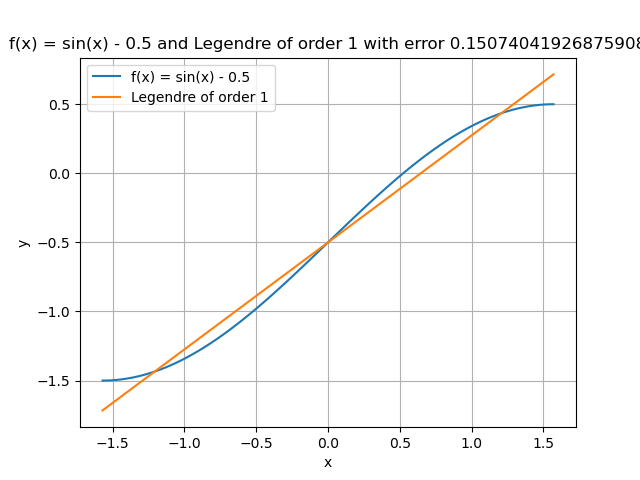
\includegraphics[width=\linewidth]{figs/Q1_d_poly_1.png}
                                    \caption{$n = 1$}
                              \end{subfigure}
                              \begin{subfigure}{0.49\linewidth}
                                    \centering
                                    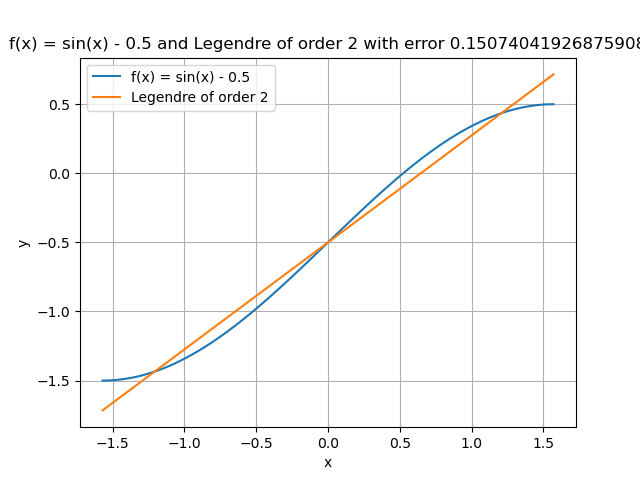
\includegraphics[width=\linewidth]{figs/Q1_d_poly_2.png}
                                    \caption{$n = 2$}
                              \end{subfigure} \\
                              \begin{subfigure}{0.49\linewidth}
                                    \centering
                                    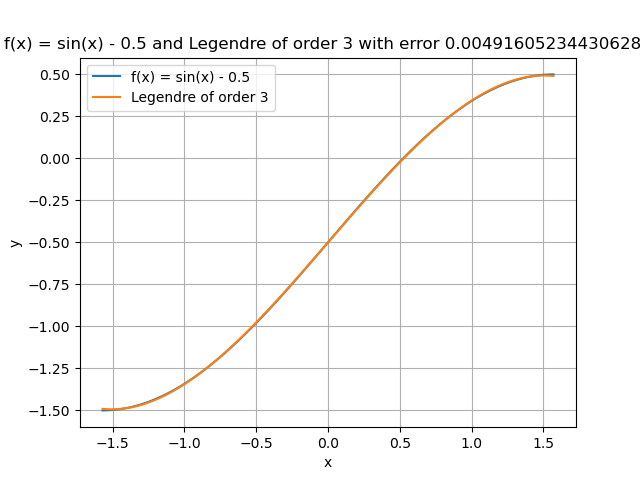
\includegraphics[width=\linewidth]{figs/Q1_d_poly_3.png}
                                    \caption{$n = 3$}
                              \end{subfigure}
                              \begin{subfigure}{0.49\linewidth}
                                    \centering
                                    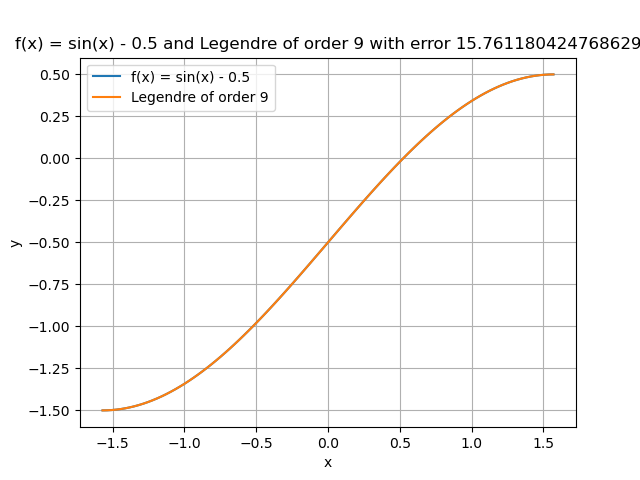
\includegraphics[width=\linewidth]{figs/Q1_d_poly_9.png}
                                    \caption{$n = 9$, complex error occurs here so they look close}
                              \end{subfigure}
                              \caption{Least Square Approximation using Legendre Polynomials}
                        \end{figure}
            \end{enumerate}
            Terminology: Suppose an approximation has error function e(x), with x in interval $[a, b]$.
            The $L_{\infty}$ error is $||e(x)||_{\infty} = \max_{a \leq x \leq b} |e(x)|$ and the $L_2$ error is $||e(x)||_2 = \sqrt{\int_a^b |e(x)|^2 dx}$.

            For your code submission, submit any code you used.

            In your pdf, please show all your hand derivations and code results, and replicate any code you would like the TAs to see.

            \clearpage
      \item Suppose very accurate values of some function $f (x)$ are given at the points $0 = x_0, x_1, \cdots , x_{100} = 1$, with the ${x_i}$ uniformly distributed over the interval [0, 1].

            (So $x_i = \frac{i}{100}, i = 0, \cdots , 100$.)

            The values $\{f (x_i)\}$ are given in the file 'problem2.txt' in sequential order

            (so, for example, $f (0.27) = f (x_{27}) = -0.964603914513021$).

            Use the method of normal equations discussed in class, to find a description of $f (x)$ as the sum of a very few polynomials and cosines and sines.
            (You may be able to guess the answer since the function is fairly simple, but please also use the method of normal equations.)

            For code, submit any code you used.
            In your pdf, replicate any code you would like the TAs to see, show your results and explain how you obtained them.
            If your search for a solution first considered some incorrect solutions, mention those and say how they informed your search for the correct solution.

                  [Hint: Try to express $f (x)$ as a linear combination of the functions, $1, x, x^2, \cdots , cos(\pi x), sin(\pi x), cos(2\pi x), sin(2\pi x), \cdots$.
                        Use the method of normal equations.
                        That method will not be enough by itself, since the underlying functions are redundant (more than a basis).
                        However, that method is useful as a subroutine in a search.
                        Try to find a very simple description of the function $f (x)$ by determining which coefficients in your sum may be
                        set to zero.
                        There may be multiple candidate answers; find one with the fewest nonzero coefficients.
                        Graphing the function may be helpful in your search.
                        You should need at most 3 nonzero coefficients when writing f (x) as a sum of the functions $1, x, x^2, \cdots , cos(\pi x), sin(\pi x), cos(2\pi x), sin(2\pi x), \cdots$.]

            \textbf{Solution:}
            \begin{lstlisting}[language=Python]
def normal_equation_method(xi: np.array, yi: np.array, n_poly: int, n_trig: int, tol: float = 1e-5):
    """Use the method of normal equations to fit a polynomial and trigonometric function to the data.

    Args:
        xi (np.array): xi data points
        yi (np.array): fi data points
        n_poly (int): number of polynomial terms
        n_trig (int): number of trigonometric terms
        tol (float, optional): tolerance for filtering out small coefficients. Defaults to 1e-5.
    """

    xi = xi.reshape(-1, 1).copy()
    yi = yi.reshape(-1, 1).copy()

    assert xi.shape == yi.shape, "xi and yi must have the same shape"

    # Construct the design matrix
    A = np.zeros((len(xi), n_poly + 2 * n_trig))
    for i in range(n_poly):
        A[:, i] = (xi**i)[:, 0]
    for i in range(n_trig):
        A[:, n_poly + i] = np.sin((i + 1) * np.pi * xi)[:, 0]
        A[:, n_poly + n_trig + i] = np.cos((i + 1) * np.pi * xi)[:, 0]

    # Use least squares to solve for the coefficients
    coeff, _, _, _ = np.linalg.lstsq(A, yi, rcond=None)

    # Filter out coefficients that are close to zero
    coeff[np.abs(coeff) < tol] = 0

    x = sp.symbols("x", real=True)

    p = 0
    for i in range(n_poly):
        p += coeff[i] * x**i
    for i in range(n_trig):
        p += coeff[n_poly + i] * sp.sin((i + 1) * sp.pi * x)
        p += coeff[n_poly + n_trig + i] * sp.cos((i + 1) * sp.pi * x)

    return sp.simplify(p), coeff
            \end{lstlisting}

            My initial guess:
            \begin{figure}[H]
                  \centering
                  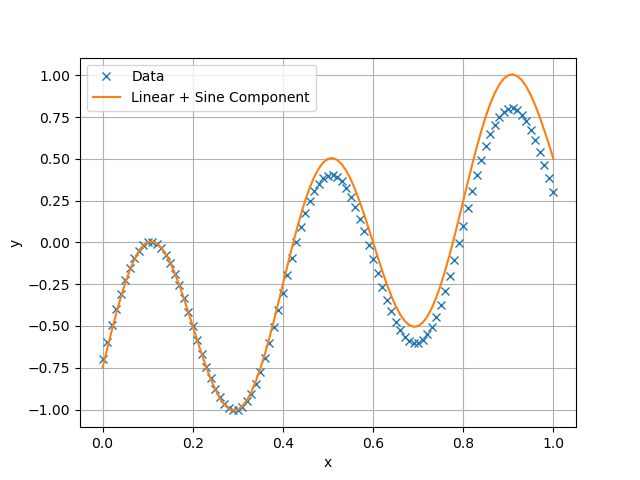
\includegraphics[width = .6\linewidth]{figs/Q2_guess.png}
                  \caption{$f(x) = 1.25 x - 0.75 + 0.625 \sin(5\pi x)$}
            \end{figure}
            The Method of Normal Equations:
            \begin{figure}[H]
                  \centering
                  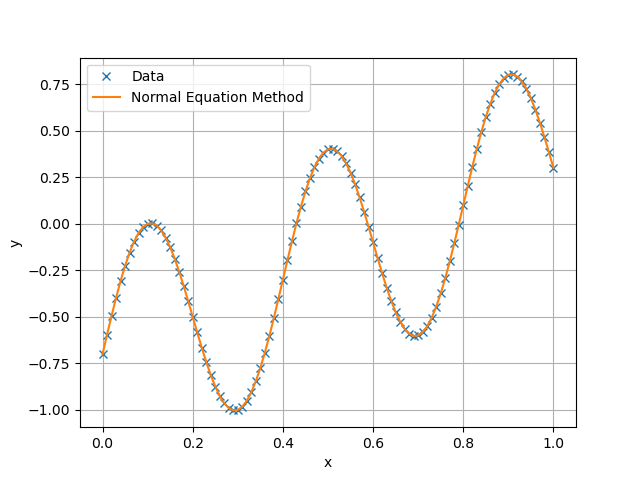
\includegraphics[width = .6\linewidth]{figs/Q2_fit.png}
                  \caption{$f(x) \approx x - 0.7 + 0.6 \sin(5\pi x)$}
            \end{figure}

            Accurate result from the method of normal equations:
            $$
                  f(x) \approx 0.999999980668295 x + 0.600000000000149 \sin(5\pi x) - 0.699999999335618
            $$

            \clearpage
      \item The Chebyshev polynomials of the first kind, $T_n(x)$, are defined indirectly on [-1, 1] by:
            \begin{align*}
                  T_n(cos \theta) = cos(n \theta), \text{for } n \geq 0
            \end{align*}
            Expanding cosine, one finds the recurrence relation $T_{n+1}(x) = 2xT_n(x)-T_{n-1}(x)$, for $n > 0$.
            \begin{enumerate}
                  \item Derive $T_4$ and $T_5$. (As always, please show your handwritten work.)

                        \textbf{Solution:}
                        \begin{align*}
                               & \begin{cases}
                                    T_0(x) & = 1 \\
                                    T_1(x) & = x
                              \end{cases} \\
                               & \Downarrow                 \\
                               & \begin{cases}
                                    T_2(x) = 2xT_1(x) - T_0(x) = 2x^2 - 1        \\
                                    T_3(x) = 2xT_2(x) - T_1(x) = 4x^3 - 3x       \\
                                    T_4(x) = 2xT_3(x) - T_2(x) = 8x^4 - 8x^2 + 1 \\
                                    T_5(x) = 2xT_4(x) - T_3(x) = 16x^5 - 20x^3 + 5x
                              \end{cases}
                        \end{align*}
                  \item Without actually computing or working out any integrals, prove that $T_4(x)$ and $T_5(x)$ are orthogonal polynomials relative to the inner product
                        $$
                              < g, h > = \int_{-1}^{1} (1 - x^2)^{-\frac{1}{2}}g(x)h(x)dx.
                        $$
                        [Hint: Look carefully at the inner product and use a property of the polynomials.]

                        \textbf{Solution:}

                        $x = \cos(\theta)$, then $dx = -\sin(\theta) d\theta$.
                        \begin{align*}
                              < T_4, T_5 > & = \int_{-1}^{1} (1 - x^2)^{-\frac{1}{2}} T_4(x) T_5(x) dx                                                         \\
                                           & = \int_{-\pi}^{0} (1 - \cos^2(\theta))^{-\frac{1}{2}} T_4(\cos(\theta)) T_5(\cos(\theta)) (- \sin(\theta)d\theta) \\
                                           & = \int_{-\pi}^{0} \frac{\cos(4\theta) \cos(5\theta)}{- \sin(\theta)} (- \sin(\theta)d\theta)                      \\
                                           & = \int_{-\pi}^{0} \cos(4\theta) \cos(5\theta) d\theta                                                             \\
                                           & = \int_{-\pi}^{0} \frac{1}{2} \left[ \cos(9\theta) + \cos(\theta) \right] d\theta                                 \\
                                           & = \frac{1}{2} \left[ \frac{\sin(9\theta)}{9} + \sin(\theta) \right] \rvert_{-\pi}^{0}                             \\
                                           & = 0
                        \end{align*}
                  \item Recall that when we have an inner product on a vector space, we may define the \textit{length of vector} v by $||v|| = \sqrt{< v, v >}$.

                        Here, we may view functions as vectors with an inner product defined by an integral
                        as above.
                        Then the length of $T_n(x)$ is the number $\sqrt{< T_n, T_n >}$.

                        It turns out that all $T_n(x)$, with $n > 0$, have the same length.

                        Prove this fact by hand-computing the length of $T_n(x)$, that is, by working out the relevant integral (leave n symbolic, assume $n > 0$).

                        (Hint: You will likely find it useful to make the substitution $x = cos \theta$ in the integral for $< T_n, T_n >$. Don't forget to change the interval of integration as well.)

                        \textbf{Solution:}

                        $x = \cos(\theta)$, then $dx = -\sin(\theta) d\theta$.
                        \begin{align*}
                              < T_n, T_n > & = \int_{-1}^{1} (1 - x^2)^{-\frac{1}{2}} T_n(x) T_n(x) dx                                     \\
                                           & = \int_{-\pi}^{0} (1 - \cos^2(\theta))^{-\frac{1}{2}} \cos^2(n\theta) (- \sin(\theta)d\theta) \\
                                           & = \int_{-\pi}^{0} \cos^2(n\theta) d\theta                                                     \\
                                           & = \int_{-\pi}^{0} \frac{1}{2} \left[ \cos(2n\theta) + 1 \right] d\theta                       \\
                                           & = \frac{1}{2} \left[ \frac{\sin(2n\theta)}{2n} + \theta \right] \rvert_{-\pi}^{0}             \\
                                           & = \frac{\pi}{2}
                        \end{align*}
                  \item Finally, show that $< T_i, T_j > = 0$ for all i and j such that $i \geq 0, j \geq 0$, and $i \neq j$.

                        (There are different ways to prove this, e.g., by working out an integral explicitly or by combining known facts from above and lecture.)

                        \textbf{Solution:}

                        $x = \cos(\theta)$, then $dx = -\sin(\theta) d\theta$.
                        \begin{align*}
                              < T_i, T_j > & = \int_{-1}^{1} (1 - x^2)^{-\frac{1}{2}} T_i(x) T_j(x) dx                                                            \\
                                           & = \int_{-\pi}^{0} (1 - \cos^2(\theta))^{-\frac{1}{2}} T_i(\cos(\theta)) T_j(\cos(\theta)) (- \sin(\theta)d\theta)    \\
                                           & = \int_{-\pi}^{0} \frac{\cos(i\theta) \cos(j\theta)}{- \sin(\theta)} (- \sin(\theta)d\theta)                         \\
                                           & = \int_{-\pi}^{0} \cos(i\theta) \cos(j\theta) d\theta                                                                \\
                                           & = \int_{-\pi}^{0} \frac{1}{2} \left[ \cos((i + j)\theta) + \cos((i - j)\theta) \right] d\theta                       \\
                                           & = \frac{1}{2} \left[ \frac{\sin((i + j)\theta)}{i + j} + \frac{\sin((i - j)\theta}{i - j}) \right] \rvert_{-\pi}^{0} \\
                                           & = 0
                        \end{align*}
            \end{enumerate}
            No code is expected or needed for any part of this problem.

            In your pdf, please show all your derivations, proofs, and handwritten work.

            \clearpage
      \item After weeks of work you have finally completed construction of a gecko robot.
            It is a quadruped robot with suctioning feet that allow it to walk on walls.
            It is also equipped with a Kinect-like sensor, providing a 3D point cloud observation of the world.
            You want to use these point clouds to reason about the environment and aid in navigation.
            \begin{enumerate}
                  \item You boot up the robot and place it on a table, taking an initial observation.
                        The observation is saved in the provided clear\_table.txt, and lists (x, y, z) locations in the following format:
                        \begin{table}[H]
                              \centering
                              \begin{tabular}{ccc}
                                    $x_1$ & $y_1$    & $z_1$ \\
                                          & $\vdots$ &       \\
                                    $x_n$ & $y_n$    & $z_n$
                              \end{tabular}
                        \end{table}
                        Points are in units of meters and the positive x-direction is right, positive y-direction is down, and positive z-direction is forward.
                        Find the least-squares approximation plane that fits the data.
                        Visualize your fitted plane along with the data.
                        What is the average distance of a point in the data set to the fitted plane?

                        \textbf{Comment:} The phrase “least-squares” is ambiguous. Below are descriptions of two possibilities that might occur to you.
                        \textbf{Please use Linear Regression.}
                        That approach is similar to our discussion of the normal equations in lecture.

                        \textbf{Orthogonal-Distance Regression:} In this approach, one computes the SVD decomposition of the $n \times 3$ matrix whose rows are the data points translated so their centroid is at the origin.
                        It turns out that the third column of V is normal to a plane that minimizes the sum of squared orthogonal distances between the translated points and the plane.
                        (This is a nice result to know.)

                        \textbf{Linear Regression:} This regression is based on the idea that, for perfectly planar data, all the points would satisfy a plane equation of the form $ax + by + cz + d = 0$.
                        So one has a natural error $\sum_i (ax_i + by_i + cz_i + d)^2$, with i indexing the data points.
                        One chooses the coefficients $\{a, b, c, d\}$ so as to minimize this error.
                        In order to avoid degeneracies, one requires that not all of $\{a, b, c, d\}$ be 0.

                        \textbf{Please use this approach.}

                        (Additional comments: (i) One convenient approach is to set one of the coefficients $\{a, b, c, d\}$ to be 1 or -1 while letting the others vary in order to compute the best plane.
                        (ii) Observe that $|ax_i + by_i + cz_i + d|$ is related to but not necessarily exactly the distance of the ith data point from the plane described by $\{a, b, c, d\}$.)

                        \textbf{Solution:}

                        We can set $d = 1$ first, then normalize the plane equation later.
                        \begin{align*}
                              ax + by + cz + 1 & = 0
                        \end{align*}
                        \begin{align*}
                              E(a, b, c) & = \sum_{i = 1}^{n} (ax_i + by_i + cz_i + 1)^2 \\
                                         & = (Ap + \mathbf{1})^T(Ap + \mathbf{1})        \\
                        \end{align*}
                        Where:
                        \begin{align*}
                              A          & = \begin{bmatrix}
                                    x_1    & y_1    & z_1    \\
                                    \vdots & \vdots & \vdots \\
                                    x_n    & y_n    & z_n
                              \end{bmatrix} \\
                              p          & = \begin{bmatrix}
                                    a \\
                                    b \\
                                    c
                              \end{bmatrix} \\
                              \mathbf{1} & = \begin{bmatrix}
                                    1      \\
                                    \vdots \\
                                    1
                              \end{bmatrix}
                        \end{align*}
                        Then:
                        \begin{align*}
                              \frac{\partial E}{\partial p} & = 2A^T(Ap + \mathbf{1}) = 0 \\
                              \Downarrow                                                  \\
                              A^T A p                       & = - A^T \mathbf{1}
                        \end{align*}
                        Solve for $p$ we get $p^* = [a^*, b^*, c^*]^T$, then the normalized plane equation is:
                        \begin{align*}
                              \frac{a^* x + b^* y + c^* z + 1}{\|p\|} & = 0
                        \end{align*}
                        \begin{lstlisting}[language=Python]
def fit_plane(points: np.array) -> np.array:
      """fit a plane with given points

      Args:
      points (np.array): in shape of (N, 3)

      Returns:
      np.array: plane coefficients in shape of (4,) and in format (a, b, c, d), normalized so ||(a, b, c)|| = 1
      """
      A = points.copy().reshape(-1, 3)

      # solve for p
      p = np.linalg.solve(A.T @ A, -A.T @ np.ones((A.shape[0], 1)))

      # Normalize the coefficients so that [a, b, c] is a unit vector
      coeff = np.append(p, 1) / np.linalg.norm(p)

      return coeff
                        \end{lstlisting}
                        Plane Equation:
                        \begin{align*}
                              -0.0951113342629671 x - 0.994246831912656 y - 0.0492653156527438 z + 0.493702932302467 = 0
                        \end{align*}
                        Average distance = 0.002740250661757354
                        \begin{figure}[H]
                              \centering
                              \begin{subfigure}{.49\linewidth}
                                    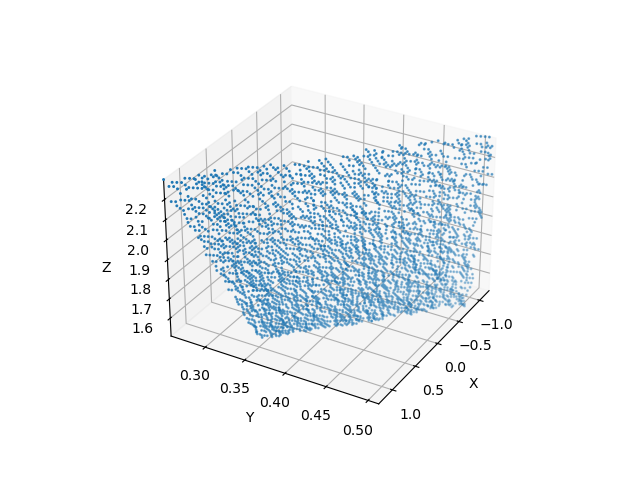
\includegraphics[width=.99\linewidth]{figs/Q4_clear_table_points.png}
                                    \caption{clear\_table.txt}
                              \end{subfigure}
                              \begin{subfigure}{.49\linewidth}
                                    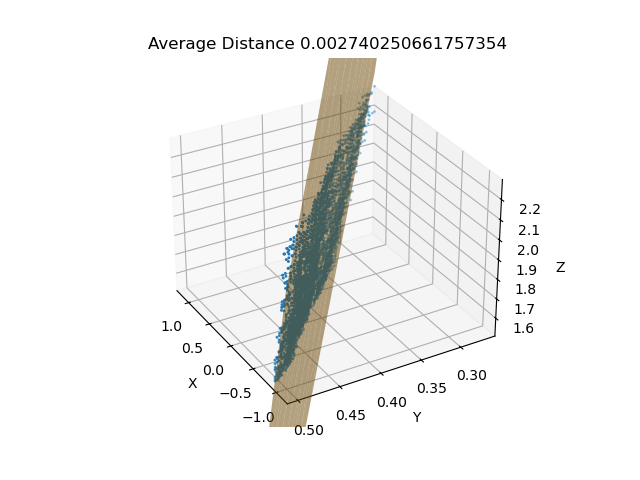
\includegraphics[width=.99\linewidth]{figs/Q4_clear_table_plane.png}
                                    \caption{Fitted Plane, note that Z axis is auto-scaled}
                              \end{subfigure}
                              \caption{Fitted Plane on clear\_table.txt}
                        \end{figure}
                  \item Interested in your gecko robot, your cat jumps up on the table.
                        You take a second observation, saved as the provided cluttered table.txt.
                        Using the same method as above, find the least-squares fit to the new data.
                        How does it look? Why?

                        \textbf{Solution:}

                        Plane equation:
                        \begin{align*}
                              -0.0975611845981769x - 0.973054533289032y - 0.208917903745619z + 0.774119219789838 = 0
                        \end{align*}
                        Average distance is 0.03741737808121337
                        \begin{figure}[H]
                              \centering
                              \begin{subfigure}{.49\linewidth}
                                    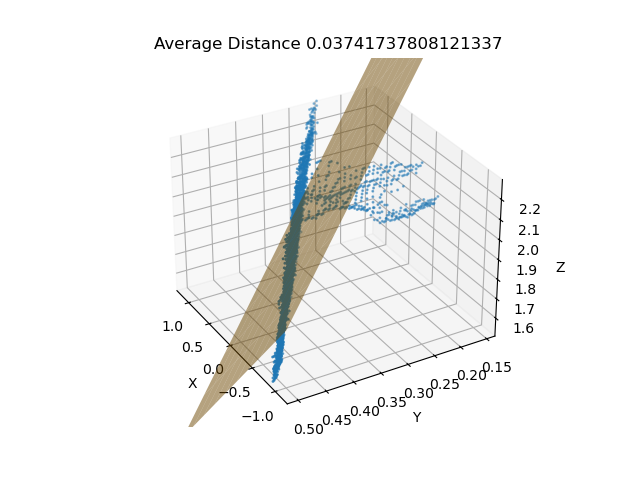
\includegraphics[width=.99\linewidth]{figs/Q4_cluttered_table_plane.png}
                                    \caption{cluttered\_table.txt}
                              \end{subfigure}
                              \begin{subfigure}{.49\linewidth}
                                    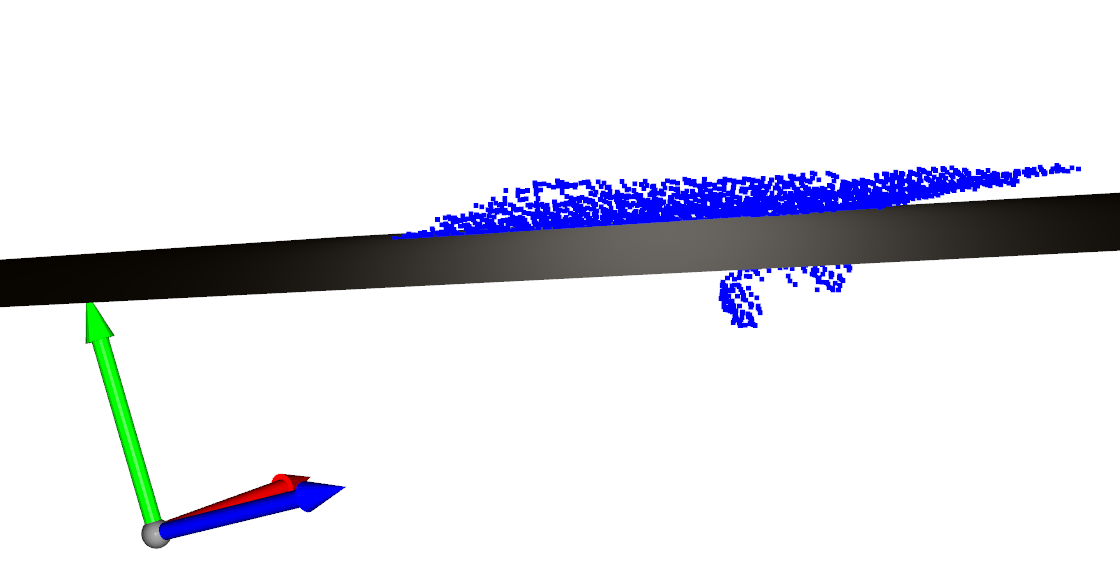
\includegraphics[width=.99\linewidth]{figs/Q4_cluttered_table_vis.png}
                                    \caption{visualization in open3d}
                              \end{subfigure}
                              \caption{Fitted Plane on cluttered\_table.txt}
                        \end{figure}
                        Well, clearly not all the points are close to the ideal plane.
                  \item Can you suggest a way to still find a fit to the plane of the table regardless of clutter?
                        Verify your idea by writing a program that can successfully find the dominant plane in a list of points regardless of outliers.
                              [Hint: You may assume that the number of points in the plane is much larger than the number of points not in the plane.]
                        Visualize cluttered\_table.txt with your new plane.

                        \textbf{Solution:}

                        RANSAC
                        \begin{lstlisting}[language=Python]
def RANSAC_fit_plane(
      points: np.array,
      max_iter: int = 10000,
      sample_ratio: float = 0.01,
      distance_inlier_threshold: float = 0.01,
) -> np.array:
      """Fit a plane to a set of noisy 3D points using RANSAC.

      Args:
            points (np.array): points in shape (N, 3)
            max_iter (int, optional): maximum iteration to perform random sampling. Defaults to 10000.
            sample_ratio (float, optional): the amount of points to sample, sample_ratio * N. Defaults to 0.01. Will not be less than 10.
            distance_inlier_threshold (float, optional): inlier points maximum average distance to their fitted plane. Defaults to 0.01.

      Raises:
            ValueError: No inlier points found.

      Returns:
            np.array: inlier points
      """
      NUM_POINTS = points.shape[0]
      SAMPLE_SIZE = max(int(points.shape[0] * sample_ratio), 10)

      inlier_index = np.array([], dtype=int)

      for _ in range(max_iter):
            # randomly sample SAMPLE_SIZE points index
            random_index = np.random.permutation(np.arange(NUM_POINTS, dtype=int))[
                  :SAMPLE_SIZE
            ]

            coeff = fit_plane(points[random_index])
            distance = average_point_to_plane_distance(points[random_index], coeff)
            if distance <= distance_inlier_threshold:
                  inlier_index = np.append(inlier_index, random_index)
                  inlier_index = np.sort(inlier_index)
                  inlier_index = np.unique(inlier_index)

      if inlier_index.size == 0:
            raise ValueError("No inlier found.")

      print(f"Inliers ratio: {inlier_index.size / NUM_POINTS}")
      return points[inlier_index]
                        \end{lstlisting}
                        Plane Equation:
                        \begin{align*}
                              -0.10068718707874x - 0.992880691307245y - 0.063639792484089z + 0.518921115704315 = 0
                        \end{align*}
                        Average distance to all the points is 0.015754165478591993

                        Average distance to table points is 0.005143845669654812
                        \begin{figure}[H]
                              \centering
                              \begin{subfigure}{.49\linewidth}
                                    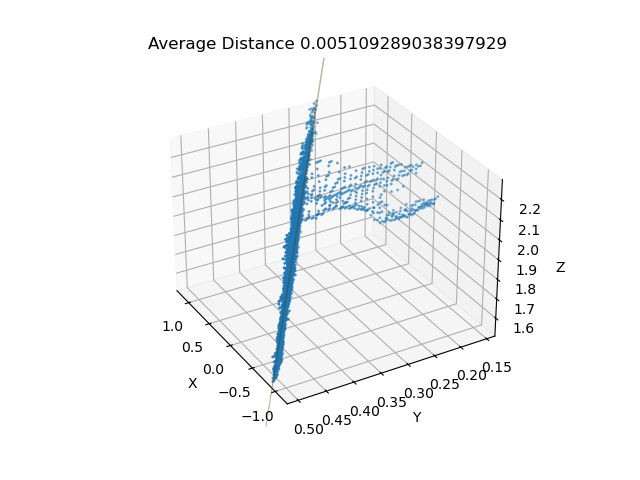
\includegraphics[width=.99\linewidth]{figs/Q4_cluttered_table_plane_ransac.png}
                                    \caption{cluttered\_table.txt RANSAC}
                              \end{subfigure}
                              \begin{subfigure}{.49\linewidth}
                                    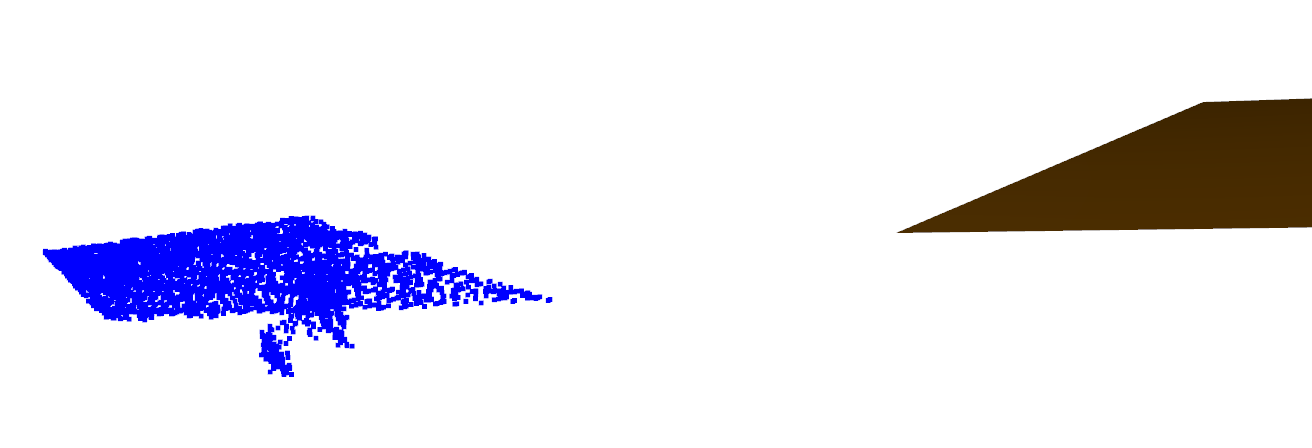
\includegraphics[width=.99\linewidth]{figs/Q4_cluttered_table_ransac_vis.png}
                                    \caption{visualization in open3d}
                              \end{subfigure}
                              \caption{RANSAC fitted Plane on cluttered\_table.txt}
                        \end{figure}
                  \item Encouraged by your results when testing on a table, you move your geckobot into the hallway and take an observation saved as the provided clean\_hallway.txt.
                        Describe an extension to your solution to part (c) that finds the four dominant planes shown in the scene, then implement it and visualize the data and the four planes.

                        You may assume that there are roughly the same amount of points in each plane.

                        \textbf{Solution:}
                        Extend the inlier criteria of RANSAC:
                        \begin{lstlisting}[language=Python]
def RANSAC_fit_plane_extended(
      points: np.array,
      num_planes: int,
      max_iter: int = 10000,
      sample_ratio: float = 0.001,
      distance_inlier_threshold: float = 0.01,
) -> np.array:
      """extended RANSAC to fit multiple planes, inlier points must satisfy:
      1. Itself is a plane with small average distance
      2. Its fitted plane must be the same plane with existing inliers
      3. The fitted plane's close to enough points (1/num_planes * 0.9)

      Args:
            points (np.array): points in shape (N, 3)
            num_planes (int): number of planes to fit, assuming each plane has roughly the same number of inliers
            max_iter (int, optional): maximum iteration to perform random sampling. Defaults to 10000.
            sample_ratio (float, optional): the amount of points to sample, sample_ratio * N. Defaults to 0.0001. Will not be less than 5.
            distance_inlier_threshold (float, optional): inlier points maximum average distance to their fitted plane. Defaults to 0.01.

      Raises:
            ValueError: No inlier points found.

      Returns:
            np.array: inlier points, might not be most points in its plane
      """
      NUM_POINTS = points.shape[0]
      SAMPLE_SIZE = max(int(points.shape[0] * sample_ratio), 5)

      print(f"Number of points: {NUM_POINTS}")
      print(f"Sample size: {SAMPLE_SIZE}")

      inlier_index = np.array([], dtype=int)

      points_homo = np.hstack((points, np.ones((points.shape[0], 1))))

      for iter in range(max_iter):
            # randomly sample SAMPLE_SIZE points index
            random_index = np.random.permutation(np.arange(NUM_POINTS, dtype=int))[
                  :SAMPLE_SIZE
            ]

            extended_index = np.unique(np.append(inlier_index, random_index))

            coeff = fit_plane(points[random_index])
            distance = average_point_to_plane_distance(points[random_index], coeff)
            extended_distance = average_point_to_plane_distance(
                  points[extended_index], coeff
            )

            all_distances = np.abs(points_homo @ coeff)
            num_inliers = np.where(all_distances <= distance_inlier_threshold)[0].size
            inliers_ratio = num_inliers / NUM_POINTS

            # print(f"inliers_ratio = {inliers_ratio}")

            # Must satisfy: itself is a plane, it's the same plane with inliers, and it has enough inliers
            if (
                  distance <= distance_inlier_threshold
                  and extended_distance <= distance_inlier_threshold
                  and inliers_ratio > 1 / num_planes * 0.9
            ):
                  inlier_index = np.append(inlier_index, random_index)
                  inlier_index = np.sort(inlier_index)
                  inlier_index = np.unique(inlier_index)

      if inlier_index.size == 0:
            raise ValueError("No inlier found.")

      print(f"Inliers ratio: {inlier_index.size / NUM_POINTS}")
      return points[inlier_index]
                        \end{lstlisting}
                        Plane Equations:
                        \begin{align*}
                              \begin{cases}
                                    0.170391902271525x - 0.984679478280239y - 0.0370529984488184z + 1.80802982578352 & = 0, \|e\| \approx 0.003144184418150686 \\
                                    -0.96366746614888x - 0.175264115206761y + 0.201562656776964z + 0.218727644397049 & = 0, \|e\| \approx 0.00451623118244317  \\
                                    -0.96403454687357x - 0.170863621367788y + 0.203575576450997z + 1.8162162422856   & = 0, \|e\| \approx 0.007681134237631346 \\
                                    0.16936975663811x - 0.984804871586362y - 0.0383829445993377z + 0.211152350861021 & = 0, \|e\| \approx 0.003350451774268799
                              \end{cases}
                        \end{align*}
                        \begin{figure}[H]
                              \centering
                              \begin{subfigure}{.49\linewidth}
                                    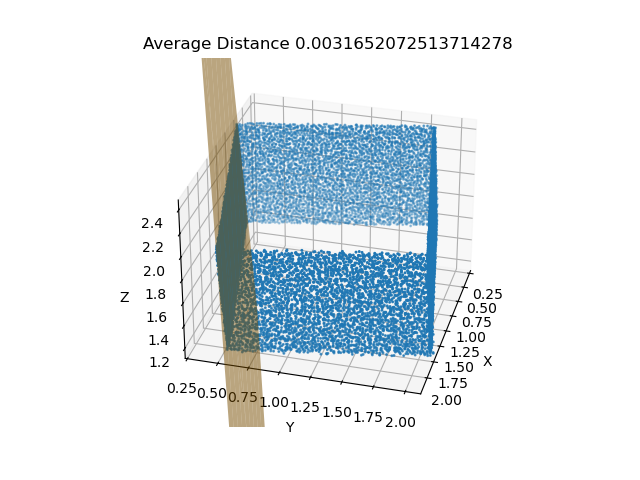
\includegraphics[width=.99\linewidth]{figs/Q4_clean_hallway_plane_ransac_1.png}
                                    \caption{clean\_hallway.txt extended RANSAC $1^{st}$ plane}
                              \end{subfigure}
                              \begin{subfigure}{.49\linewidth}
                                    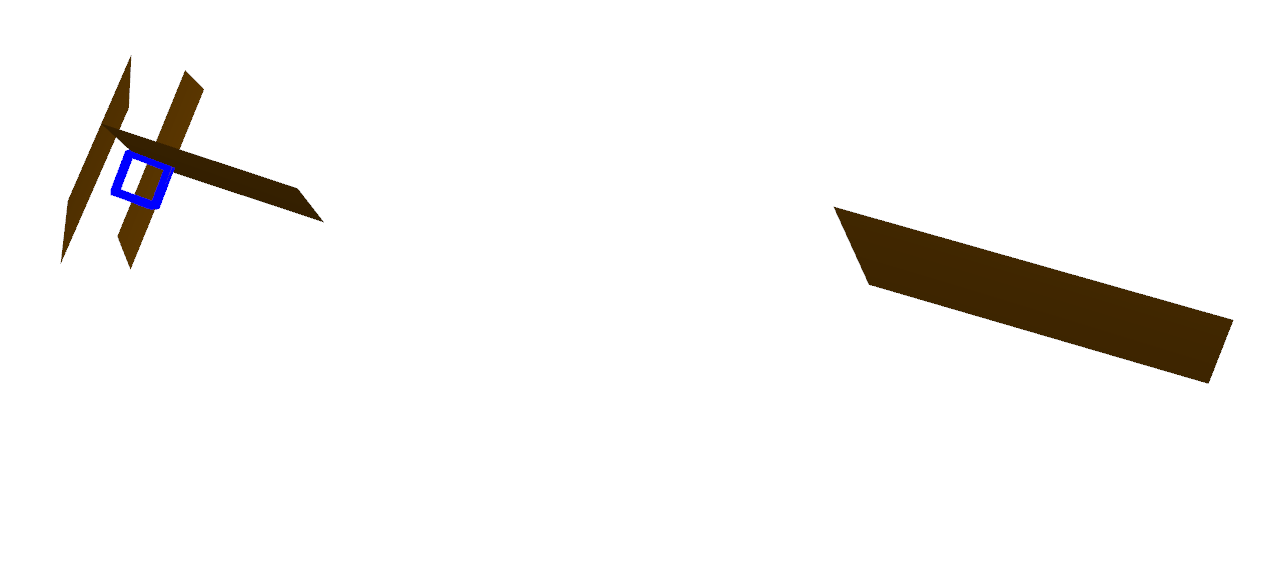
\includegraphics[width=.99\linewidth]{figs/Q4_clean_hallway_extended_ransac_vis_all.png}
                                    \caption{visualization of all planes in open3d}
                              \end{subfigure}
                              \caption{extended RANSAC fitted plane on clean\_hallway.txt}
                        \end{figure}
                        More results available in the \textit{figs/} folder.
                  \item You decide it is time to test your gecko robot's suction feet and move it to a different hallway.
                        The feet are strong enough to ignore the force of gravity, allowing the robot to walk on the floor, walls, or ceiling.
                        However, the locomotion of the legs works best on smooth surfaces with few obstacles.
                        Using your solution from part (d), describe how you can mathematically characterize the smoothness of each surface.
                        Load the provided scan cluttered\_hallway.txt, find and plot the four wall planes, describe which surface is safest for your robot to traverse, and provide the smoothness scores from your mathematical characterization.

                        Note that you may no longer assume that there are roughly the same amount of points in each plane.

                        \textbf{Solution:}

                        I characterize the smoothness of each surface by the variance of distance between all the points to the fitted plane, lower variance indicates higher smoothness.
                        \begin{lstlisting}[language=Python]
def voxel_downsample_point_cloud(points, voxel_size):
    """
    Downsamples the input point cloud using a voxel grid filter.

    Args:
        points (np.array): Input points in shape (N, 3).
        voxel_size (float): The size of the voxel grid.

    Returns:
        np.array: Downsampled points in shape (M, 3).
    """
    # Create Open3D point cloud
    pcd = o3d.geometry.PointCloud()
    pcd.points = o3d.utility.Vector3dVector(points)

    # Downsample
    downsampled_pcd = pcd.voxel_down_sample(voxel_size)

    # Extract NumPy array
    downsampled_points = np.asarray(downsampled_pcd.points)

    return downsampled_points
                        \end{lstlisting}
                        RANSAC is modified to consider inlier points only if their fitted plane is close to enough number of points (threshold is adaptive).
                        \begin{lstlisting}[language=Python]
def RANSAC_fit_multiple_planes(
      points: np.array,
      num_planes: int,
      max_iter: int = 10000,
      sample_size: int = 5,
      distance_threshold: float = 0.01,
      inlier_ratio: float = 0.9,
):
      """Fit multiple planes to a set of 3D points using RANSAC.

      Args:
            points (np.array): Points in shape (N, 3).
            num_planes (int): Number of planes to fit.
            max_iter (int, optional): Maximum iterations for RANSAC. Defaults to 10000.
            sample_size (int, optional): number of points to sample for every RANSAC iteration. Defaults to 5.
            distance_threshold (float, optional): Distance threshold for inliers. Defaults to 0.01.
            min_inliers (int, optional): Minimum number of inliers to accept a plane. Adjust as needed.

      Returns:
      """
      points = points.copy().reshape(-1, 3)
      remaining_points = points.copy().reshape(-1, 3)

      planes = []

      for i in range(num_planes)[::-1]:
            print(f"Fitting plane {i + 1}...")

            min_inliers = int(remaining_points.shape[0] / (i + 1) * inlier_ratio)

            inlier_indices = np.array([], dtype=int)
            # Can no longer assume the same number of inliers for each plane
            for _ in range(max_iter):
                  # Randomly sample points
                  sample_indices = np.random.permutation(
                  np.arange(remaining_points.shape[0], dtype=int)
                  )[:sample_size]
                  extended_index = np.unique(np.append(inlier_indices, sample_indices))
                  sample_points = remaining_points[sample_indices]

                  # Fit a plane to the sample points
                  plane_coefficients = fit_plane(sample_points)

                  fit_distance = average_point_to_plane_distance(
                  sample_points, plane_coefficients
                  )
                  inlier_distance = average_point_to_plane_distance(
                  remaining_points[extended_index], plane_coefficients
                  )

                  all_distances = np.abs(
                  remaining_points @ plane_coefficients[:3] + plane_coefficients[3]
                  )
                  num_inliers = np.where(all_distances <= distance_threshold)[0].size

                  if (
                  fit_distance <= distance_threshold
                  and inlier_distance <= distance_threshold
                  and num_inliers >= min_inliers
                  ):
                  inlier_indices = np.append(inlier_indices, sample_indices)
                  inlier_indices = np.sort(inlier_indices)
                  inlier_indices = np.unique(inlier_indices)

            if inlier_indices.size > 0:
                  print(f"Found {inlier_indices.size} inliers.")
                  coeff = fit_plane(remaining_points[inlier_indices])

                  # find all points that are close to this plane in points
                  distance_all_points = np.abs(points @ coeff[:3] + coeff[3])
                  point_close_to_this_plane = points[
                  np.where(distance_all_points <= distance_threshold)
                  ]
                  distance_close_to_this_plane = distance_all_points[
                  np.where(distance_all_points <= distance_threshold)
                  ]
                  print(f"Points close to this plane: {point_close_to_this_plane.shape[0]}")
                  planes.append(
                  {
                        "coeff": fit_plane(point_close_to_this_plane),
                        "mean_distance": distance_close_to_this_plane.mean(),
                        "var_distance": distance_close_to_this_plane.var(),
                        "var_distance_all": distance_all_points.var(),
                        "points": point_close_to_this_plane,
                        "num_points": point_close_to_this_plane.shape[0],
                  }
                  )

                  # remove all points close to this plane from remaining points
                  distance_remaining_points = np.abs(remaining_points @ coeff[:3] + coeff[3])
                  remaining_points = remaining_points[
                  np.where(distance_remaining_points > distance_threshold)
                  ]

                  print(f"Remaining points: {remaining_points.shape[0]}")

      # Sort planes by number of points
      planes = sorted(planes, key=lambda x: x["num_points"], reverse=True)

      return planes
                        \end{lstlisting}
                        Some results:
                        \begin{figure}[H]
                              \centering
                              \begin{subfigure}{.49\linewidth}
                                    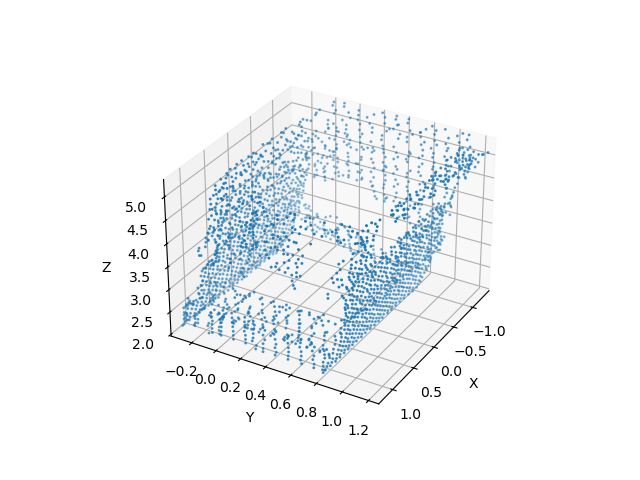
\includegraphics[width=.99\linewidth]{figs/Q4_cluttered_hallway_downsampled.png}
                                    \caption{cluttered\_hallway.txt downsampled}
                              \end{subfigure}
                              \begin{subfigure}{.49\linewidth}
                                    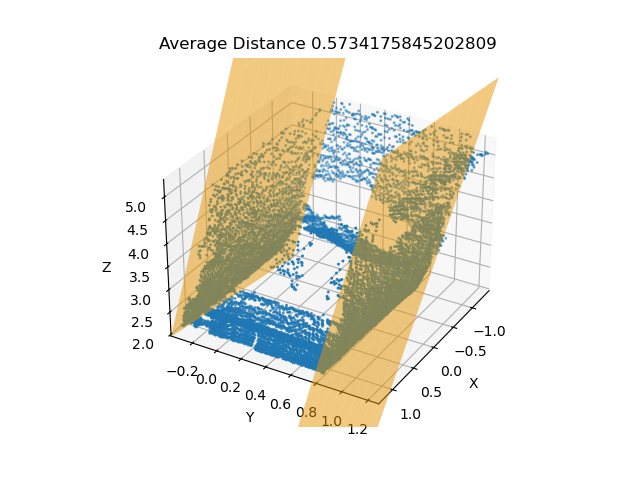
\includegraphics[width=.99\linewidth]{figs/Q4_cluttered_hallway_planes.png}
                                    \caption{cluttered\_hallway.txt RANSAC visualized with original point cloud}
                              \end{subfigure}
                              \caption{RANSAC fitted plane on cluttered\_hallway.txt}
                        \end{figure}
                        The algorithm turns to be very fragile to parameter changes, e.g., sample size, distance threshold.

                        There could be better metric, e.g., project close points to the fitted plane and see if there are holes, to prevent fitting a densely scanned ring instead of a plane.

                        Anyway, here are the 2 best plane in terms of smoothness and number of points:
                        \begin{align*}
                              \begin{cases}
                                    0.0180113772483563x + 0.995495709171525y - 0.0930799834051354z + 0.534986213611912 & = 0, \|e\| \approx 0.0039050967482275882 \\
                                    -0.0134299102483403x - 0.994749138160533y + 0.101458314787885z + 0.582350784438808 & = 0, \|e\| \approx 0.0035446492378242746
                              \end{cases}
                        \end{align*}
            \end{enumerate}
            Parts (c), (d), and (e) intentionally leave room for some creativity and design.
            There may be several good approaches.

            Please submit code for all parts (a), (b), (c), (d), (e) of this problem.
            In your pdf, explain what you did, how to run your code, and what results you obtained.
            Describe any design decisions you made.
            Include as well in your pdf any images you used to visualize data, and explain their meanings.
            Finally, replicate in your pdf any code you would like the TAs to see.
\end{enumerate}

\end{document}
